%
% File naaclhlt2018.tex
%
%% Based on the style files for NAACL-HLT 2018, which were
%% Based on the style files for ACL-2015, with some improvements
%%  taken from the NAACL-2016 style
%% Based on the style files for ACL-2014, which were, in turn,
%% based on ACL-2013, ACL-2012, ACL-2011, ACL-2010, ACL-IJCNLP-2009,
%% EACL-2009, IJCNLP-2008...
%% Based on the style files for EACL 2006 by 
%%e.agirre@ehu.es or Sergi.Balari@uab.es
%% and that of ACL 08 by Joakim Nivre and Noah Smith

\documentclass[11pt,a4paper]{article}
\usepackage[hyperref]{naaclhlt2018}
\usepackage{times}
\usepackage{latexsym}
\usepackage{graphics, graphicx}
\usepackage{url}
\usepackage{todonotes}
\usepackage{amsmath}
\aclfinalcopy % Uncomment this line for the final submission
%\def\aclpaperid{***} %  Enter the acl Paper ID here

%\setlength\titlebox{5cm}
% You can expand the titlebox if you need extra space
% to show all the authors. Please do not make the titlebox
% smaller than 5cm (the original size); we will check this
% in the camera-ready version and ask you to change it back.

\newcommand\BibTeX{B{\sc ib}\TeX}

\title{Empirical Evaluation of LSTM Language Models \bigskip
on Syntactic Dependencies}



\author{
Maartje de Jonge\\
\tt Student ID: 194107\\
{\tt maartjedejonge@gmail.com} \\\And
David Rau \\
\tt Student ID: 17725184\\
{\tt david.rau@student.uva.nl} \\}


\date{}

\begin{document}
\maketitle

\begin{abstract}

\noindent 

% main idea
- language model, number agreement

% key findings
- able to learn the numbers of nouns and verbs
- modest sensitivity to syntactic structure

\end{abstract}


%----------------------------------------------------------------------------------------
%	INTRODUCTION
%----------------------------------------------------------------------------------------
\section{Introduction}

%%%%%%%%%%% Problem Area: RNN, LSTM networks
Neural networks have become increasingly popular
for the task of language modeling.
While feed-forward networks only take into account
a fixed history of preceeding words to predict the next word,
standard recurrent neural networks (RNN) and 
Long Short-Term Memory (LSTM) network architectures
have the ability to capture long-distance statistical regularities.
The access to potentially unlimited history 
has resulted in substantial improvements 
in perplexity and error rates
compared to feed-forward networks~\cite{Mikolov2010,Sundermeyer2013}. 

%%%%%%%%%%% Context: What do we already know
Regularities in natural language are often sensitive to syntactic structure.
RNNs and LSTMs are sequence models that do not explicitly
incorporate syntactic structure,
capturing such dependencies is therefore challenging.
Linzen et al.~\ref{Linzen2016} investigate the capability
of LSTMs to learn syntactic dependencies, taking
number agreement in noun-verb dependencies as an example.
%They compare the performance of
%a general LSTM language model with the performance of 
%LSTM models trained on explicit grammatical targets.
%They conclude that LSTMs can capture 
%structure-sensitive dependencies given explicit supervision;
%while the language modeling objective is not sufficient for learning
%such dependencies.
Their results show that the language modeling objective by itself
is not sufficient for learning structure-sensitive dependencies;
and that more explicit supervision is required.

%%%%%%%%%%% Problem + Approach
In this paper we investigate an LSTM language model
in more detail to get a better insight into what 
information these models actually encode.
We consider statistic, syntactic and semantic information
and analyse how the model uses this information
to establish number agreement. 
We take an empirical approach.
That is, we treat the model as a black box
and learn about it by observing its behavior
in carefully designed experiments.

%%%%%%%%%%% Results
The results show that ...

%\paragraph{Outline}
%The remainder of this report is organized as follows \ldots

%We first repeat the experiments from the linzen paper
%on a language model trained on PTB corpus.
%We reach similar conclusions,
%TODO: what about distance?
%While the model can establish number agreement
%for simple cases without intervening nouns,
%it fails for more complex cases scoring below average.

%We then take a closer look on the errors
%it made on simple cases without intervening nouns.
%By analyzing noun/verb combinations
%we identify verbs that show a strong preference for either
%one of the forms (singlar or plural),
%ignoring the count of the noun.
%In addition, we identified nouns that
%the model seems to have failed to learn or even mis-learned
%the number.
%We explained these cases by frequency statistics on the training corpus.

%We then look at syntactic information exposed 
%by function words such as 'that' and 'of'.
%We measure the performance of the model on 
%generated sentences constructed following a specific
%syntactic structure. 
%From this experiment we learned that
%function words can help the model to establish
%number agreement with the structurally relevant noun.
%But the evidence is very week.

%Thus far we looked at random generated nonsense
%sentences, ignoring the fact that sentences 
%are typically about something.
%In real world sentences some verbs 
%tend to form subject verb dependencies with certain nouns
%while other nouns do not mae sense.
%This can help the model.
%The price of the products stabilize/stabilizes.
%prices are semanticly related to stabilize,
%while products are not.
%We compare prefixes with a noun that
%is semantically related 
%compare with same prefic with noun replaced by random noun.
%to prefixes with a noun that is not.
%Does the semantic relation helps to establish
%number agreement with the relevant noun?

%From these experiments we conclude that
%...


%----------------------------------------------------------------------------------------
%	BACKGROUND
%----------------------------------------------------------------------------------------



%A background section, in which you explain what is language modelling,
%what kind of language model you studied, and what is the problem you
%focus on. To write this background section, you can use the suggested
%papers, but also add papers;

%----------------------------------------------------------------------------------------
%	PREVIOUS WORK
%----------------------------------------------------------------------------------------

\section{Related Work}
\label{related work}

%summary of ~\citep{Linzen2016}

%Linzen 2016

%%%% Research Question
LSTM
- can capture long distance statistical regularities
- do not explicitly incorporate syntactic structure
- question: can LSTM capture dependencies that follow from syntactic structure, from a corpus without syntactic annotations?
- more specific: investigate number agreement in English subject-verb dependencies
as an example of a structure sensitive dependency

%%%% Experiments
- train models with different training objectives
  - with explicit grammatical target as training objective
    - number prediction
    - verb infliction
    - grammatical judgement
  - a more generic language model with the objective to predict the next word
- corpus: wikipedia

- evaluate how these models perform on simple and more complex sentences:
  - simple cases: noun that is the subject closeby verb, no intervening nouns
  - effect of long distance: lot of words inbetween noun and verb
  - complex cases: intervening nouns with different number inbetween head of subject noun and verb
  
%%%% Results
- high or reasonable overall accuracy for all models, explained by the fact that most real world sentences are actually simple (no attractors)
   - NP, VI, GJ, LM
- all explicitly trained language models perform reasonable on complex cases.
   - distance
   - attractors
- language model performs bad on complex cases. sensitive to most recent noun.
  - more complex objective, lack of data? no, google also fails.

%%%% Detailed analysis of results
More detailed error analysis shows that
- function words are important, by comparing with a baseline model trained on noun verb sequences
- relative clauses are challenging, especially when relativizer misses
- some errors in identifying nouns (due to ambiguity: drives) and identifying the number of a noun

- activations: units that track main subject, subject of current clause, embedding status, number of main clause subject/most recent noun

%%%% Conclusion
- LSTM can capture grammatical structure given targeted supervision
- language modeling is insufficient for capturing syntax sensitive dependencies
- authors advice: supplement language modeling objectives with more explicit targets
for tasks in which it is desirable to capture syntactic dependencies.


%----------------------------------------------------------------------------------------
%	EXPERIMENTS
%----------------------------------------------------------------------------------------

\section{Replication}
\label{replication}

In this section we replicate some experiments of~\citep{Linzen2016} to get a general impression of how well our model is able to establish number agreement.
All experiments in this paper are performed using an LSTM model
trained on a general language modeling task\footnote{
\url{https://github.com/pytorch/examples/tree/master/word_language_model}
}.

\subsection{Singular and Plural Nouns}

\textbf{Data:} 
The language model was tested on lower case sentences that were generated from the Wall Street Journal section of the Penn Treebank \citep{Marcus1993}. Therefore, 40 nouns and verbs, that were amongst the most common and occur in the test corpus as well as in the language model's corpus, were extracted. Those words build the base for the sentence generation for the subsequent experiments. 

\textbf{Model evaluation:} In order to evaluate the performance of our model, we query it with sentences containing both, the plural (\ref{sent:wrong}) and the singular (\ref{sent:right}) mode of the verb: 

\begin{equation}
	\label{sent:wrong}
	\textnormal{the producer plan}
\end{equation}
\begin{equation}
	\label{sent:right}
	\textnormal{the producer  \textbf{plans}}
\end{equation}
Following the experiments in \citep{Linzen2016} we examine the models error rate predicting the number of a verb. That is, the model receives the words leading up to the verb and needs to decide between the singular and plural forms of a particular verb.
%We examine sentences with a given number of nouns of opposite number intervening %between the subject and the verb. 

    \begin{figure}
    \centering
        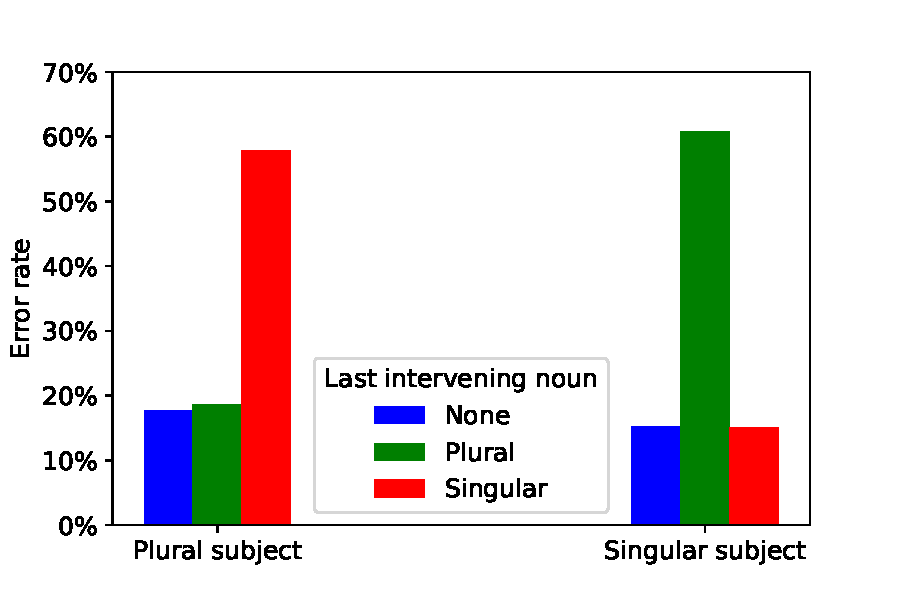
\includegraphics[scale=0.5]{2b.pdf}
            	\caption{Error rates of the language model plotted against: presence and number of last intervening noun}
        \label{fig:2b}
    \end{figure}
    ~ %add desired spacing between images, e. g. ~, \quad, \qquad, \hfill etc. 
      %(or a blank line to force the subfigure onto a new line)
    \begin{figure}
    \centering
        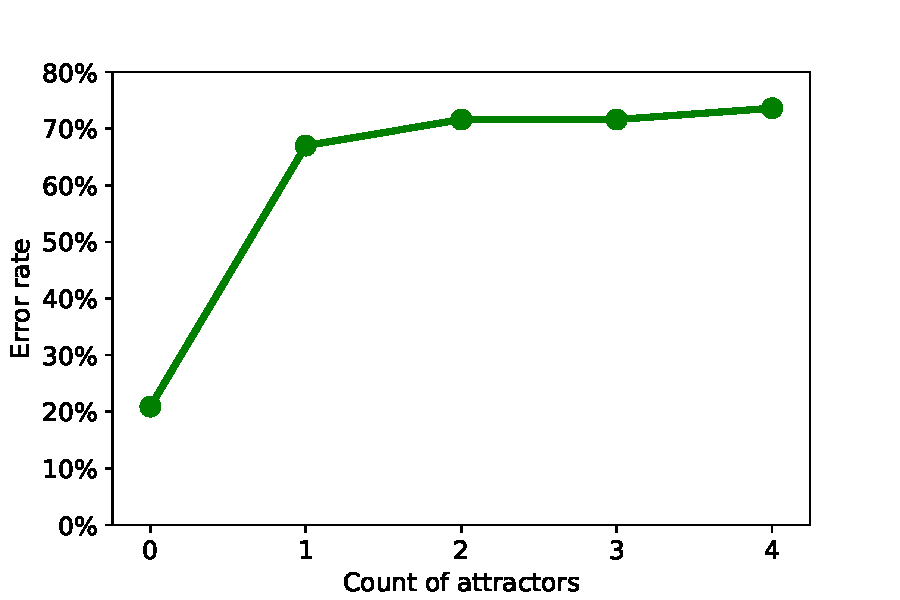
\includegraphics[scale=0.5]{2c.pdf}
        \label{fig:2c}
            \caption{Error rates of the language model plotted against count of attractors in dependencies with homogeneous intervention.}
    \end{figure}

We first test how the model's ability to predict the number of the verb is affected by none and one intervening noun, respectively. If there is an intervening noun we keep track whether the number of the noun differs from the number of the subject. If it does so it is referred to as an \textit{agreement attractor}. In this way we can easily spot whether the model makes use of the most obvious heuristic: choosing the the number of the verb only in dependence of the last intervening noun in the sentence.

As depicted in Figure \ref{fig:2b} our model performs slightly worse for plural subjects (17.7\% error rate) than for singular (15,2\% error rate) when no intervening nouns are present. An intervening noun with the same number as the subject causes a slight increase of the error rate to 18.6\% and a decrease to 15.1\%, respectively. However, when the number of the subject differs from the intervening noun the error rates increased dramatically; in singular subjects to 57,9\% in plural subjects to 60,8\%. The fact that it performs worse than predicting the number by chance implies that the model indeed predicts the number of the verb in dependence of the last noun and therefore fails to find the dependency between verb and noun.

\subsection{Multiple Attractors}

In the following we examine the error rate when adding multiple attractors to the sentence. In order to avoid the model of being distracted by an intervening noun with the same number as the subject we only insert nouns with the same number. Linzen et al.~\citep{Linzen2016} refer to such as  \textit{ dependencies with homogeneous intervention}. Consider the following example sentences:
\begin{equation}
	\label{sent:right2}
	\textnormal{the \textbf{interest} in the \underline{shares} of the \underline{businesses} \textbf{rises} \dots}
\end{equation}
\begin{equation}
	\label{sent:wrong2}
	\textnormal{the \textbf{interest} in the \underline{shares} of the \textit{business} \textbf{rises} \dots}
\end{equation}
In (\ref{sent:right2}) the underlined represent homogeneous interventions, whereas in (\ref{sent:wrong2}) the number of the intervening nouns differ. The bold words highlight the dependency between noun and corresponding verb.

Figure \ref{fig:2c} shows that with an increasing number of noun interventions the error rate goes from 20.8\% (0 attractors) up to 73.6\% (4 attractors) which is worse than randomly guessing the number of the verb. 

%TODO: describe 2b_least in text and give implications

\section{Own Experiments}
\label{own-experiments}
To predict the correct number of a given verb,
the language model should be able to
1. identify the noun that is the head of the subject for the verb
2. establish the number of the noun (non-trivial since no knowledge of -s postfix for plurals)
3. establish the number of the given verb forms (also non-trivial).

In the first sub section we investigate if our model is able to
do this for simple cases with only a single noun in the prefix.
%
In the second sub section we investigate if our model can handle
more complex cases with two nouns in the prefix,
and what information it then uses to identify the head of the subject.

%TODO: describe model (or in previous section)

\subsection{Noun-Verb Agreement in Simple Cases}

In this section we further investigate the ability of the model to
establish number agreement for nouns and verbs in the simplest case
following the pattern: ``The <noun> <verb>''. Notice that
the determiner ``The'' clearly indicates the position of the subject.
From this we hope to get insights whether or not the model is sensitive to noun-verb agreement, i.e. if the model tends to predict plural verbs for plural nouns and singular verbs for singular nouns.


Using the 40 most frequent nouns and verbs that we already used earlier in the replication section, we generated 80 x 40 sentences. To evaluate how the language model is going to perform on these sentences we tested, for each noun-verb combination, how likely the model is going to predict the singular and the plural verb respectively.

As a result of this evaluation we obtained a matrix in which the entries indicate the models preference for the singular/plural verb. We calculate each value
\begin{equation}
	v = P(<VBP>)/ P(<VBP> + P(<VBZ>), 
\end{equation}
where P is the models prediction probability, <VBP> is the plural verb and <VBZ> the singular verb. In this manner the matrix provides a ratio for singularity ($v=0$) and plurality($v=1$). We call $v$ the \textit{plurality preference}. The upper part of the matrix contains all noun-verb combinations for the singular nouns, whereas the lower part contains the plural nouns. 

In order to get a better visual impression we sorted the columns after the sums of the columns. The rows were sorted in a similar manner, but separately in order to conserve the separation between singular (upper half) and plural (lower half) nouns. The resulting matrix is shown in Fig. \ref{fig:matrix_ratio}.

As we expected the majority of the verbs in the upper half of the matrix are predicted correctly to be singular with a high certainty. The same for the lower, plural half. Overall it can be said that around the horizontal axis as well as at the vertical borders we can observe that there are specific verb/noun combinations for which the model is rather uncertain. This also matches our expectations that there are regions in the matrix where the model is not clearly in favour of the singular or plural verb. 

In the following we will investigate the two special cases of verbs and nouns where the model is less certain: 
In the columns close to the left border of the matrix, we can find verbs of which the model prefers the plural verb over the singular, regardless the number of the subject. For example the verb `buy` in column 0 has a plurality preference of 0.95. In the far right columns we find the verbs of which the plural verb is preferred over the singular. The verb `say` in column 39 has a plurality preference value of 0.1625.

There are also nouns which clearly prefer one number over another. Around the middle of the matrix we can observe a few words that are clearly predicted wrong most of the times. The noun `income` with a plurality rate of 0.15 is mostly predicted singular whereas for example the words `weeks` (0.9) column 40, `months` (0,9) column 41, `years` (0,85) column 43, `days` (0,7) column 44, are predicted plural most of the times.

    
To investigate the impact of the frequencies in the training data on the plurality rate (and therefore on the error) further, we calculated the error rate for each noun and plotted it against the frequency of the same noun. We expected a high error rate for low frequent nouns. As the Fig. \ref{fig:noun_freq_error} shows there is no clear evidence that a low frequency of singular or plural nouns in the training data leads to wrong predictions of the model. Figure \ref{fig:noun_freq_error} shows that there are singular as well as plural nouns with a low count that are predicted correctly most of the times (error rate < 0.2).

 
    \begin{figure}
    \centering
        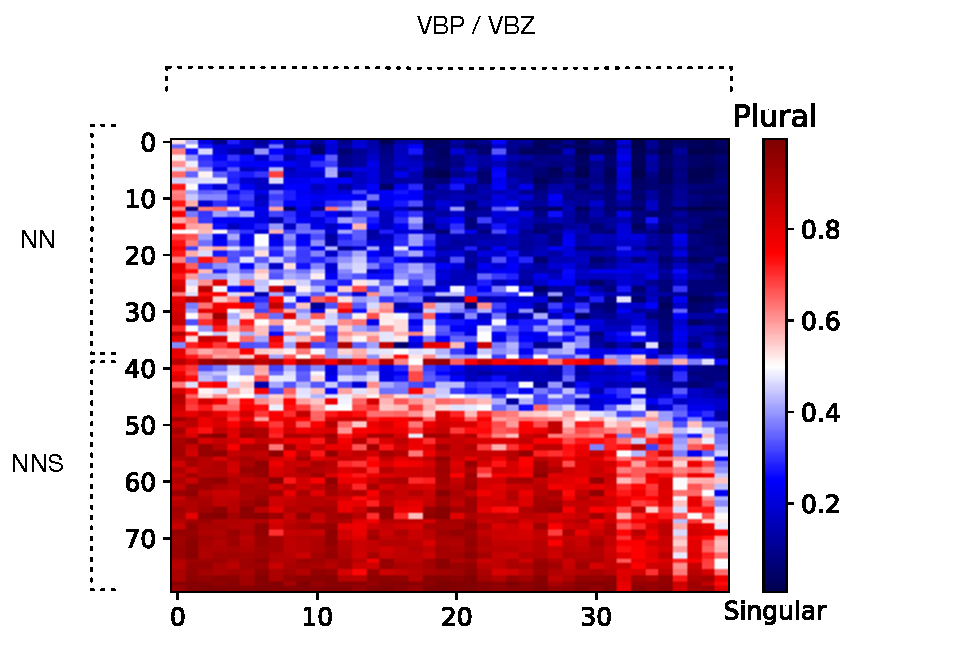
\includegraphics[scale=0.5]{matrix_plot_ratio.pdf}
        \label{fig:matrix_ratio}
        \caption{Singularity/plurality ratio for 80 x 40 sentences (generated from the most frequent 40 nouns and verbs). The upper half contains the singular nouns (NN), the lower half contains the plural nouns(NNS). A red cell indicates a plural preference for a specific word/noun combination, whereas a blue cell indicates a singular preference. }
    \end{figure}
    ~ %add desired spacing between images, e. g. ~, \quad, \qquad, \hfill etc. 
      %(or a blank line to force the subfigure onto a new line)
     \begin{figure}
     \centering
        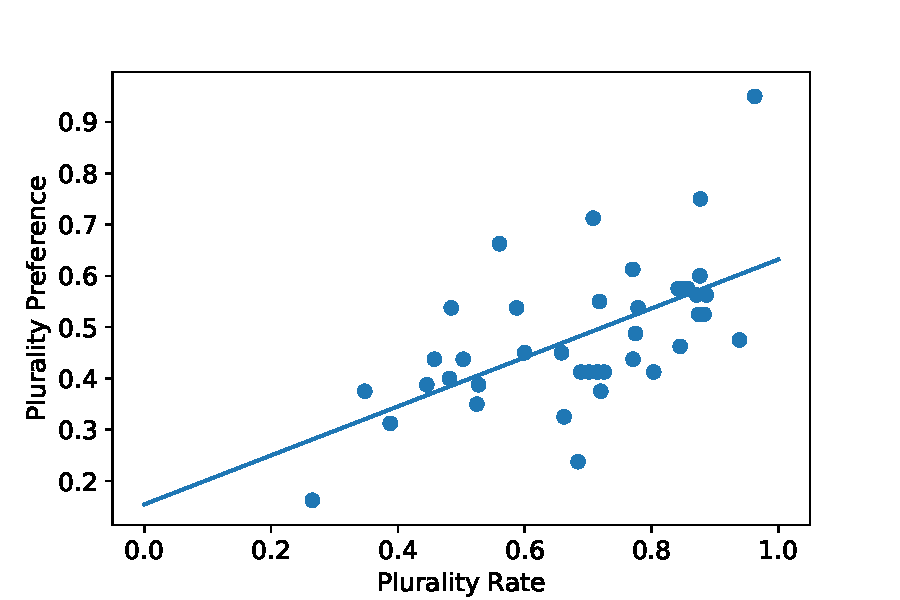
\includegraphics[scale=0.5]{lin_reg.pdf}
        \caption{Plurality rate plotted against the plurality preference of the model for all nouns. The line arises from a linear regression through the points. }
        \label{fig:lin_reg}
    \end{figure}
         \begin{figure}
          \centering
        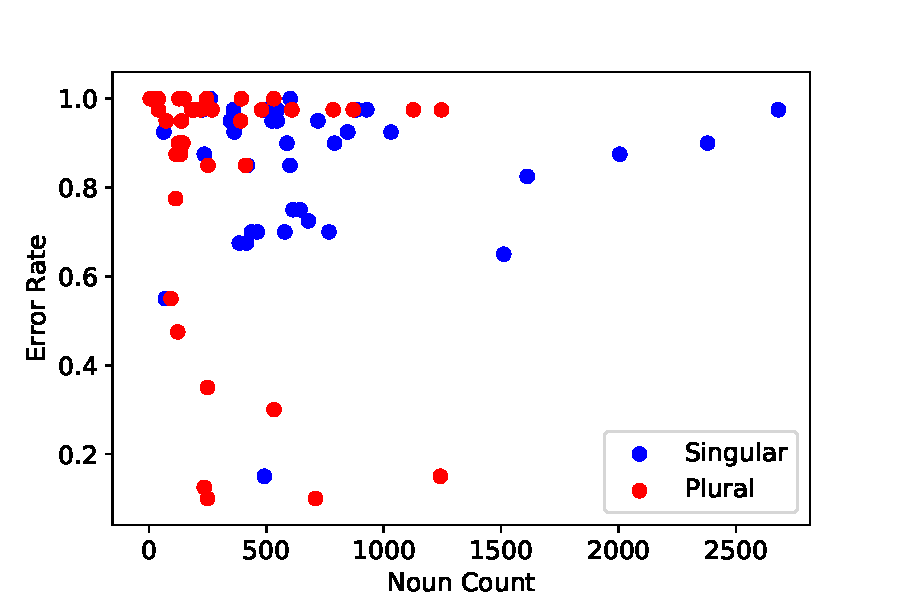
\includegraphics[scale=0.5]{noun_freq_error_rate.pdf}
        \caption{Influence of the noun frequency on the error rate of the model.}
        \label{fig:noun_freq_error}
    \end{figure}
    
    
The previous experiment neglects the fact that even though a word is frequent in the corpus it could never be the subject in the training sentence. We investigated whether the nouns that we encountered before as being predicted wrong most of the times, namely: `weeks`,`months`, `years` and `days` are in fact rarely the subject in the training data. This suggests that the model is indeed not able to establish the number agreement for nouns and verbs in a more general but rather in a statistical way. Figure \ref{fig:lin_reg} supports this assumption. It shows the plurality rate plotted against the plurality preference for each verb. We can see that with an increasing plurality rate the plurality preference increases, as expected. The line in the figure was generated by performing a linear regression through the points. 



\subsection{Noun-Verb Agreement in Complex Cases}

In Section \ref{replication} we analysed the performance of the model
on complex sentences, containing one or more 
nouns.
The results show that the model is very
sensitive to the most recent noun,
performing worse-than-chance with only one single attractor.
%(Figure \ref{fig:2c}). 

In this section we investigate whether
syntactic and semantic information
can still help the model 
to establish number agreement
in case of multiple nouns.
We focus on sentences with exactly two nouns
of opposite number.


\subsubsection{Syntactic Information}

%%%%% OBJECTIVE
Function words such as `that' or `of' carry 
important information about the syntactic structure of a sentence.
In this Section we investigate if the model
uses this information to establish number agreement
for complex sentences.

%%%% TEST DATA
We generated sets of sentence prefixes using 
different syntactic templates.
An example is ``The \_ of the \_''
We instantiate these templates by randomly
picking two nouns and a verb 
from a set of frequently used nouns and verbs. 
Each combination of nouns and verbs instantiates
two prefixes that differ by their plurality.
For example ``The company of the governments''
and ``The companies of the government'',
with the option to choose between the verb forms
`know' and `knows'.
Since the nouns and verbs are randomly picked,
the generated prefixes 
are typically not semantically
meaningful.

We generated 2 x 1000 sentences per template,
for a total of 11 templates.
The sentences for each template are constructed using the same
noun and verb combinations.
We defined 7 templates for which the first noun is 
the head of the subject (table \ref{tab:attractor_templates}),
while 4 templates have the second noun as the head of the subject
(table \ref{tab:lastnoun_templates}).
The templates were defined after a manual inspection
of sentences from the corpus.

%%%% EXPERIMENT:
We evaluate how the model responds to the generated test inputs.
That is, for each test prefix we let the model decide between 
the singular and plural form of the given verb. 
We measure the error rate for each template.
However, instead of showing the error rates we
show how much the language model tends to agree with the most recent noun.
This corresponds to the error rate for the templates in table \ref{tab:attractor_templates},
while it corresponds to accuracy for the templates in table \ref{tab:lastnoun_templates}.
Showing the `last noun agreement rate' makes it easier
to compare the behavior of the model for different templates.

%%%% ANALYSIS:
The results are shown in Figure \ref{fig:last_noun_rates},
using green and red colors to indicate if 
the last noun is actually the head of the subject (green)
or not (red). 
%
We see that all bars are above the 0.5 rate,
which shows that the model is most
likely to agree with the last noun,
even in cases where this is syntactically incorrect. 
%
We also see that the red bars are slightly
lower than the green bars,
0.67 compared to 0.79 on average.
This shows that the model is even more likely
to prefer the last noun if this is
also syntactically correct.
This suggests that the model has 
at least some sensitivity
to syntactic information carried by function words.
%

%
We further discuss two special cases,
namely the first red bar (T1) and 
the last green bar (T11).
T1, ``the \_ and the \_ '', is a special case because it 
actually contains two singular nouns
instead of one singular and one plural noun. 
The predicted verb should be plural because of the
conjunction word `and'.
The existence of two singular nouns 
makes it hard for the model
to pick the plural verb,
which could explain the high error rate
for T1 in Figure \ref{fig:last_noun_rates}.
%
T11 uses different templates for the singular 
(the \_ 's \_ ) and the plural (the \_' \_) possessive form.
The last green bar in Figure \ref{fig:last_noun_rates} shows the average result.
We suspect that the relatively low accuracy
in this case might be explained by the infrequent
occurrence of the plural possessive form in written text.
Indeed, a closer inspection of the numbers showed that
the singular template had an accuracy
of 0.77 (compared to 0.71 for all singular prefixes), 
while the accuracy of the plural template
was lower, namely 0.66 (compared to 0.63 overall for plural prefixes).
%

%%%% DISCUSSION / CONCLUSION:
We conclude that, although the model 
performs poorly on syntactically complex sentences it
still shows some sensitivity for syntactic 
information exposed by function words. 


\begin{figure}
    \centering
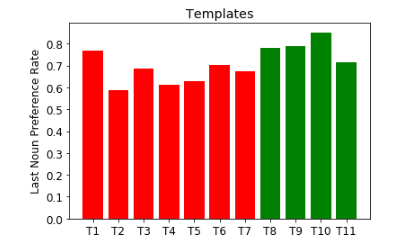
\includegraphics[scale=0.5]{screenshot-syntactic-templates} 
\caption{Preference rates for agreement to the last noun.
The colors indicate whether this is syntactically correct (green)
or incorrect (red).
}
%TODO: save picture instead of making screenshot 
%TODO title Templates below
\label{fig:last_noun_rates}
\end{figure}



\begin{table}[t] 
\parbox{\linewidth}{
\centering
\begin{tabular}{ l l r }
  T1    & the \_ and the \_     &  0.77 \\
  T2    & the \_ in the \_      &  0.59 \\
  T3    & the \_ by the \_      &  0.69 \\
  T4    & the \_ of the \_      &  0.61 \\
  T5    & the \_ near the \_    &  0.63\\
  T6    & the \_ at the \_      &  0.70\\
  T7    & the \_ without the \_ & 0.67  \\
\end{tabular}
\caption{Templates for which the number of the verb 
is opposite to the number of the last noun} 
\label{tab:attractor_templates}
}
\end{table}


\begin{table}[t] 
\parbox{\linewidth}{
\centering
\begin{tabular}{ l l r }
  T8    & the \_ the \_         &  0.78\\
  T9    & the \_ that the \_    &  0.79\\
  T10   & the \_ whether the \_ &  0.85\\
  T11   & the \_ 's \_ (for plural: the \_' \_)          &  0.72 \\
\\
\\
\\
\end{tabular}
\caption{Templates for which the number of the verb 
corresonds to the number of the last noun} 
\label{tab:lastnoun_templates}
}
\end{table}


\subsubsection{Semantic Information}

We now look at semantic clues, i.e. companies
are more likely to produce than employees.
We investigate if the model is able to establish
number agreement between the verb and the semantic related noun,
ignoring the non-semantic related attractor noun.
  
1. TEST DATA:
We construct a testset (100+ sentences) consisting of pairs with singular and plural prefixes, in the following format  
``The NN of the NNS ...[VBZ/VBP]'' and
``The NNS of the NN ...[VBZ/VBP]'' 
whereby the head of the subject (the first noun)
is semantically related to the verb, while the attractor (the second noun)
is randomly picked. An example is:
``The prices of the employee ...[stabilizes/stabilize]'' and 
``The price of the employees ...[stabilizes/stabilize]''.

In addition we construct a comparison set consisting of the same prefixes
(same verb and attractor noun),
but with the difference that the first noun is also randomly picked and
therefore most likely not semantically related. Example:
``The newspapers of the employee ...[stabilizes/stabilize]'' and 
``The newspaper of the employees ...[stabilizes/stabilize]''.


EXPERIMENT:
Evaluate our model on the constructed testset and on the comparison set.
If the model scores significantly better on the testset
then it shows sensitivity to semantic clues.

%(remark: we can repeat the experiment with the nouns interchanged and check that we %score worse now,
%e.g. "The employee that the prices ... [stabilize/stabilizes]" 
%In that case syntax and semantics are inconsistent)

HOW TO FIND CO-OCCURRENCE RATIOS
We use PMI to measure associations between verbs and nouns.
%(https://en.wikipedia.org/wiki/Pointwise_mutual_information#Applications)


\begin{itemize}
\item find all nouns (NN) and verbs (VBZ) in a tagged corpus 
(sec02-21.gold.tagged).
(pick a random selection if all is too much
but make sure you are not only looking at
frequent verbs since they tend to be general like 'is/are'
instead of specific like 'stabilize')
\item  build a matrix with nouns as rows and columns as verbs
\item  fill entries with Count('noun and verb co-occur in a sentence')
i.e. loop over all sentences and add one if noun and verb exists in sentence
(or use skip grammar, but only count noun that appears before verb, see also lab4)
\item  Also keep track of the total occurrences for the Verbs and nouns
\item replace each enty by the PMI calculated from the 
co-occurrence count, the total occurences of the noun, and the occurences
of the verb
\item select for each column the entry with the highest score(s)
(you may ignore very general verbs like is/are)
\end{itemize}

Remark: can be learned from tagged data set, no need to look at training data








%----------------------------------------------------------------------------------------
%	CONCLUSION
%----------------------------------------------------------------------------------------
\section{Conclusion and Future Work}
\label{conclusion}


%\todo[prepend]{This is a subtle one.
%I think Linzen considers simple cases not to be proof of capturing 
%grammatical structure,
%since they can be solved by simple last noun agreement. However,
%I basically agree with you that learning counts and recognizing nouns
%and verbs are also grammatical achievements. 
%In addition, Linzen is negative over general LSTM language models 
%because he contrasts those with his explicitly trained grammatical LSTM models.
%Anyway, I would probably not refer to Linzen here in this way.
%}
Overall, we conclude that LSTM language models
are able to capture grammatical properties to some extend.
Our model was able to predict the correct number of noun/verb pairs 
for most of the simple sentences;
from which we conclude that it does encode the plurality number of those words. 
Through further analysis of the models decisions in the simplest cases, we could find some evidence that the model occasionally falls back to statistical properties of the training corpus, such as word frequencies.
This may happen for example when the ratio between the plural 
and the singular form of a verb is biased.

On more complex cases, e.g. sentences containing intervening nouns 
of opposite number
in between the subject and the verb, 
the model most often fails to establish number agreement. 
In this case we could observe that the model at least shows 
some sensitivity for syntactic information.
That is, the model is most likely to agree with the
most recent noun, but it is a bit less likely to do so 
in case this is syntactically incorrect.

For future work it would be interesting to perform similar experiments on real world sentences rather than on artificially constructed ones. 
The sentences that we generated are typically not semantically meaningful,
in addition, they are syntactically less divers than real world sentences. 
It remains an open question whether our model would perform differently on those.

An interesting aspect of analysing LSTMs is to look into the embeddings and further investigate the internal state of the network rather than treating it like a black box. Looking at the activations of the LSTMs might give further insights into the strenghts and weaknesses of the model and could lead to a better error analysis then by looking solely at the predictions. 

To follow up on the experiments it would also be interesting to train the model with explicit syntactic structures instead of relying too much on statistical properties of the training corpus.





% include your own bib file like this:
%\bibliographystyle{acl}
%\bibliography{naaclhlt2018}
\bibliography{article}
\bibliographystyle{aaai-named}

\end{document}
